\section{Introduction}
\label{sec:introduction}
The goal of this project is to propose a first version of electronics and logic design to readout a directional radiation sensor (see sec. \ref{sec:radiation_sensor}) using an ASIC (Application Specific Integrated Circuit) (see sec. \ref{sec:asic}).
A non-negligible part of the work was the gathering and exchange of information between PSI and eSpace.
The following report should serve as a good basis for a final design of the sensor interface and also provides more precise data on a systems level.

\subsection{Mission Overview: Tantalum Project}
\label{sec:mission_overview}
The directional radiation sensor is part of a cubesat mission placed in GTO (Geostationary Transfer Orbit).
The scientific goal is to gather more precise data about the radiation environment in the Van Allen belts and it's impact on the lifetime of a satellite.

The following scientific instruments will be implemented in the 3U or 6U cubesat:\cite{tantalumproject2016}
\begin{itemize}
	\item EDSS and SDSS (RUAG)
	\item Directional Radiation Sensor (PSI)
	\item Solar Cell Experiment (AZUR SPACE)
\end{itemize}


\subsection{Space Environment}
\label{sec:space_environment}
The environment a spacecraft encounters during operations is composed of four physical components:\cite{hastings2004spacecraft}
\begin{itemize}
	\item Neutral Gas Environment
	\item Plasma Environment
	\item Radiation Environment
	\item Particulate Environment
\end{itemize}

Only the radiation environment is explained further in this report, since it has a major impact on the directional radiation sensor and it's electronics.
It's effects and modulation is also the main purpose of this mission.

\subsubsection{Radiation Environment}
\label{sec:radiation_environment}
``The radiation environment has two components: electromagnetic and corpuscular. 
The electromagnetic radiation environment includes the ambient solar photon flux, that reflected (and emitted) from the Earth, and the electromagnetic interference (EMI) generated by the operation of spacecraft systems or arcing.
It also includes electromagnetic waves generated by the plasma environment and photons emitted from spacecraft nuclear sources.
The corpuscular radiation environment consists of the ambient flux of particles (electrons, protons, heavy ions, and neutrons) and any high-energy particles emitted by nuclear sources or reactors.''\cite{hastings2004spacecraft}

The Tantalum Project will mainly focus on the study of the ambient flux of particles.
RUAG's system will measure the quantity of electrons with their EDSS (Electron Detector Subsystem) and the quantity of protons, and heavy ions with their SDSS (Stacked Detector Subsystem).
The directional radiation sensor from PSI will mainly concentrate on the electrons and their directionality.\footnote{This is due to the fact that protons and heavy ions have larger energy densities then electrons and therefore usually need multiple stacked detectors to be detected.}
The solar cell experiment from AZUR SPACE will study the degradation effect of the radiation environment on different types of solar cells.

\subsubsection{Van Allen Belts}
\label{sec:van_allen}
The Van Allen radiation belts are the two main radiation belts around Earth (see fig. \ref{fig:van_allen_belts}).
They are composed of energetic charged particles, mostly originating from the solar wind, that have been trapped in the Earth's magnetic field.
The inner Van Allen belt (1'000 to 6'000 km above the Earth) is mainly dominated by protons with energies exceeding 100 MeV but also has high concentrations of electrons in the range of hundreds of keV.
The outer Van Allen belt (13'000 to 60'000 km above the Earth) consists mainly of high energy electrons in the range of 0.1 to 10 MeV.\cite{wikipedia2016vanallen}

\begin{figure}[H]
    \centering
    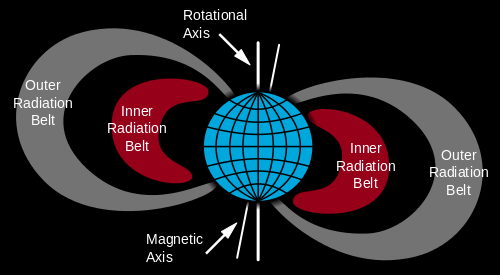
\includegraphics[width=0.5\textwidth]{van_allen_belts.png}
    \caption[Van Allen Radiation Belts]{Cross section of the Van Allen radiation belts.\cite{wikipedia2016vanallen}}
    \label{fig:van_allen_belts}
\end{figure}


\subsection{Directional Radiation Sensor}
\label{sec:radiation_sensor}
A typical radiation sensor is composed of a simple diode (see fig. \ref{fig:detector_diode}).
Reverse biasing of this diode will induce a depletion region in which ionizing particles can be detected.
The passing of such a particle generates charges (electron-hole pairs) in the depletion region, which produce a signal under the action of an electric field.
Since the amount of energy needed to create electron-hole pairs is only dependent on the detector material, the number of created charges can be calculated and therefore the energy of the radiation can be deduced.\cite{rossi2006pixel}

\begin{figure}[H]
    \centering
    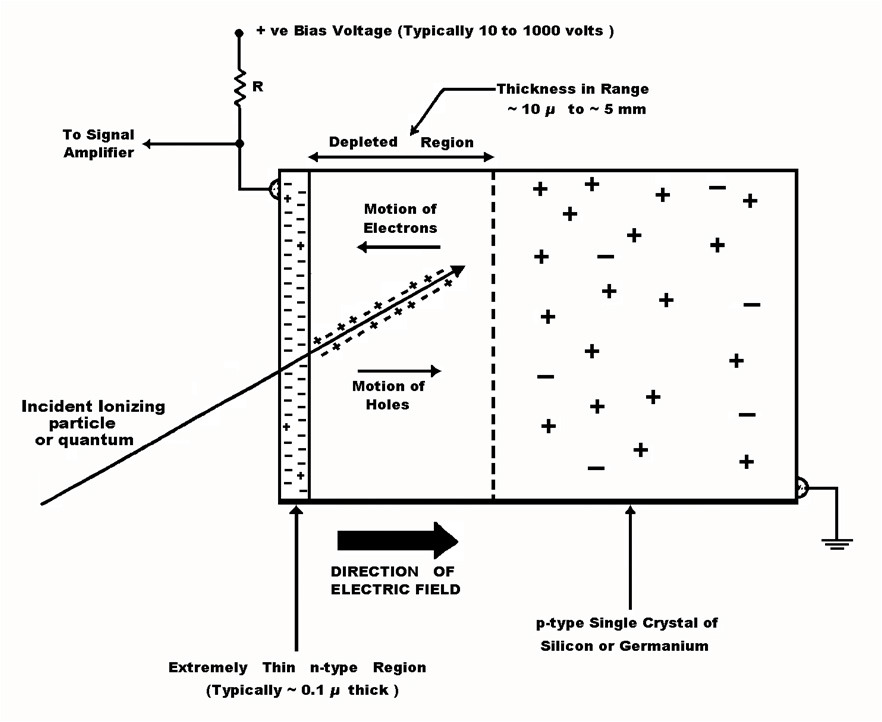
\includegraphics[width=0.5\textwidth]{detector_diode.png}
    \caption[Schematic Detector Diode]{Schematic plot of a single detector diode.\cite{am2016semiconductor}}
    \label{fig:detector_diode}
\end{figure}

The sensor from PSI (see fig. \ref{fig:detector_die}) is a PIPS (Passivated Implanted Planar Silicon) detector.\footnote{The sensor is similar to the one used in the RADEM instrument of the JUICE mission.}
It consists of 31 reverse biased diodes (PN junctions), meaning that their anode should be set to 80V and their cathode to GND.
A copper, dome-shaped stencil (see fig. \ref{fig:detector_stencil}) is used to shield most of the detector from radiation.
Holes in the stencil will enable radiation to fall onto the detector diodes, which are shaped in a way that the wholes project on an equal surface.\footnote{Hence the tear shape of the outer diodes and the round shape of the center diode.}
The whole circular area around the diodes are used as a large anode, it's purpose is to smoothen the electric field lines in the detector junctions and around them.
This is to avoid noise from charges created outside of the detectors and therefore inside the large anode, which are collected and removed using a capacitance.
Guard rings are placed around the large anode, they protect the detectors from leakage current.
The back of the die is connected to a large ground pad, while the detectors, large anode and guard rings are connected via wire-bonding to a PCB.

\begin{figure}[h!]
    \centering
    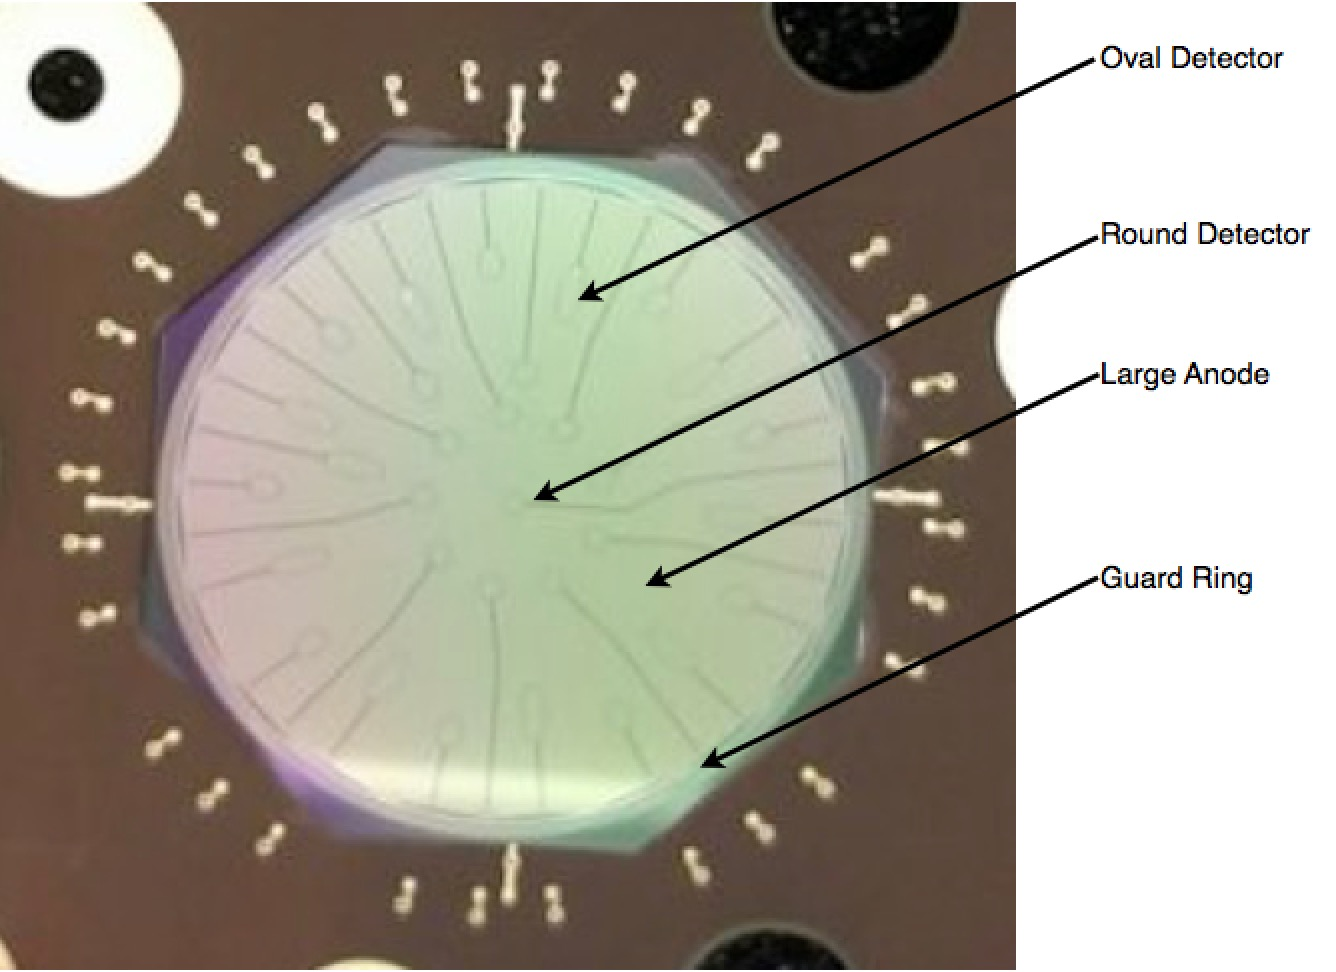
\includegraphics[width=0.5\textwidth]{detector_die.jpg}
    \caption[PSI Detector Die]{Picture of the PSI detector die.}
    \label{fig:detector_die}
\end{figure}

\begin{figure}[h!]
    \centering
    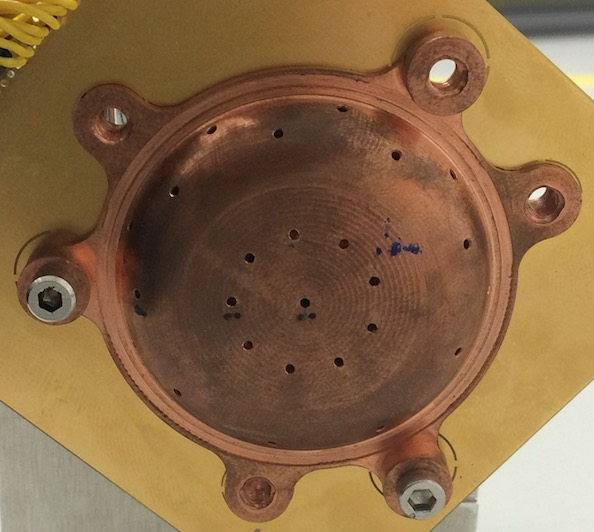
\includegraphics[width=0.5\textwidth]{detector_stencil.jpg}
    \caption[PSI Detector Stencil]{Picture of the PSI detector stencil.}
    \label{fig:detector_stencil}
\end{figure}
